\documentclass{article}
\usepackage{mysettings}

\title{Relazione Progetto di Machine Learning \\Classificazione di lettere dell'alfabeto ASL}
\author{Habasescu Alin Marian}

\begin{document}

\maketitle

\tableofcontents
\clearpage

\section{Descrizione del Progetto}

L'obiettivo di questo progetto è progettare un sistema di classificazione in 
grado di identificare lettere statiche dell'alfabeto americano dei segni (ASL) a partire da immagini 
di dimensione \(28\times28\) pixel. Le lettere \(Y\) e \(Z\) sono escluse dall'analisi poichè 
richiedono movimento per essere rappresentate. 

Sono stati considerati e confrontati diversi modelli di Machine Learning affontati durante il corso, al fine 
di identificare il modello che ottiene i migliori risultati in ternini di accuratezza e capacità di generalizzazione.

\begin{itemize}

    % TODO: VANNO SPIEGATI DI PIU' I VARI MODELLI ?

    \item \textbf{Naive Bayes}: Un classificatore probabilistico sul teorema di Bayes e sull'assunzione
    di indipendenza tra le features.
    \item \textbf{MLPClassifier}: Una rete neurale a più strati che utilizza funzioni di attivazione 
    non lineari per apprendere pattern complessi dalle immagini di input.
    \item \textbf{Support Vector Machine (SVM)}: Un algoritmo di classificazione che trova un iperpiano 
    ottimale che separa le classi. 
    \item \textbf{Decision Tree}: Un modello basato su una struttura ad albero, che suddivide i dati in 
    base a regole decisionali sequenziali. 
\end{itemize}

\paragraph{Metodologia}
Il progetto segue i seguenti passi principali: 
\begin{enumerate}
    \item  \textbf{Caricamento e visualizzazione dei dati}.
    \item  \textbf{Preprocessing dei dati}.
    \item  \textbf{Addestramento dei modelli} e \textbf{valutazione dei modelli}.
    \item  \textbf{Analisi dei Risultati ottenuti}.
\end{enumerate}

\section{I Dataset}

Nel progetto si utilizzano due dataset distinti per l'addestramento e la valutazione dei modelli. 

Questi dataset vengono caricati dai file CSV forniti tramite la funzione \texttt{load\_datasets}, che suddivide i dati in \textit{features} 
(valori dei pixel delle immagini) e \textit{target} (le lettere corrispondenti). 

La funzione \texttt{visualize\_dataset} consente invece di analizzare i dati caricati, mostrando un'anteprima 
grafica delle prime osservazioni sotto forma di immagini \(28\times28\) pixel in scala di grigi e associandole 
alle lettere dell'alfabeto ASL (0\-25, mappati su A\-Z).

Il dataset di training è composto da \(27455\) campioni, mentre il dataset di test contiene \(7172\) campioni. 
Ogni campione rappresenta un'immagine di una lettera statica dell'alfabeto ASL, accompagnata dai valori 
di grigio relativi ai 784 pixel che costituiscono l'immagine.

\begin{figure}[H]
    \centering
    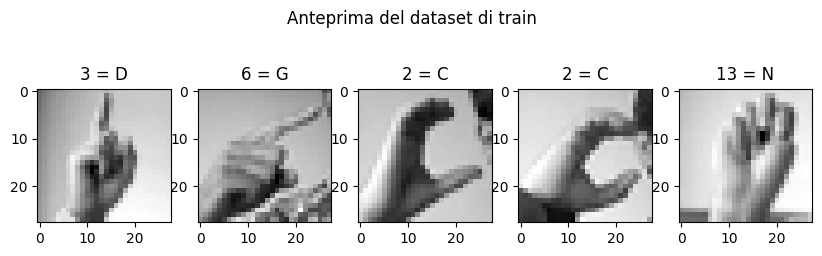
\includegraphics[scale=0.5]{"Figures/output.png"}
    \label{fig:dataset}
\end{figure}

\begin{figure}[H]  
    \centering
    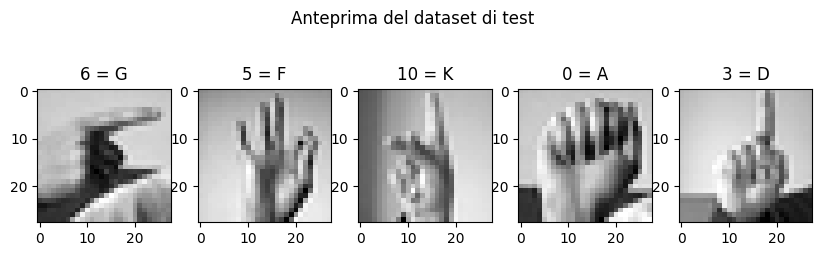
\includegraphics[scale=0.5]{"Figures/output1.png"}
    \label{fig:dataset_test}
\end{figure}

\section{Analisi Esplorativa dei Dati (EDA)}

Dopo il caricamento dei dataset, viene eseguita una serie di operazioni per analizzare le caratteristiche dei dati.

\begin{itemize}
    \item \textbf{Distribuzione delle classi}: Verifica di un bilanciamento uniforme tra le classi.
    \item \textbf{Distribuzione dei valori dei pixel}: Analisi della gamma di valori di pixel (0-255) per 
    determinare la necessità di normalizzazione.
\end{itemize}    

\begin{figure}[H]
    \centering
    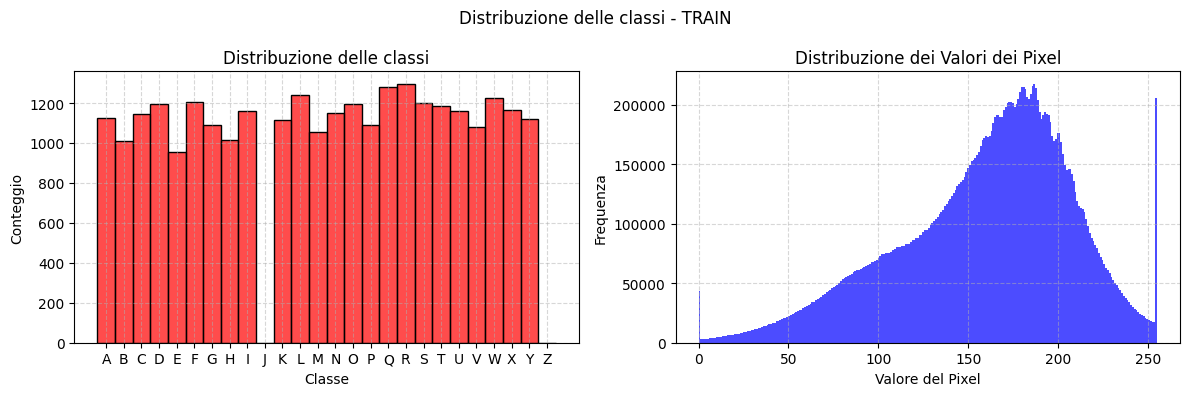
\includegraphics[scale=0.5]{"Figures/output2.png"}
    \label{fig:dataset}
\end{figure}

Durante l'analisi esplorativa dei dati, non sono stati osservati evidenti squilibri nella distribuzione delle classi, 
evinziando però valori prossimi a 255 per la distribuzione dei pixel.

\section{Preprocessing dei dati}

I dati sono stati normalizzati utilizzando lo \textbf{StandardScaler} per ottimizzare 
l'addestramento dei modelli. 

\section{Addestramento dei modelli e metriche di valutazione}

Sono stati addestrati i seguenti modelli: 

\begin{itemize}
    \item \textbf{Naive Bayes}: Un classificatore probabilistico sul teorema di Bayes e sull'assunzione
    di indipendenza tra le features.
    \item \textbf{MLPClassifier}: Una rete neurale a più strati che utilizza funzioni di attivazione 
    non lineari per apprendere pattern complessi dalle immagini di input.
    \item \textbf{Support Vector Machine (SVM)}: Un algoritmo di classificazione che trova un iperpiano 
    ottimale che separa le classi. 
    \item \textbf{Decision Tree}: Un modello basato su una struttura ad albero, che suddivide i dati in 
    base a regole decisionali sequenziali. 
\end{itemize}

\paragraph{Metriche di valutazione}
\begin{itemize}
    \item \textbf{Accuracy}: Rappresenta la percentuale di campioni correttamente classificati.
    \item \textbf{Classication Report}: Precision, Recall e F1-Score per ogni classe.
    \item \textbf{Confusion Matrix}: Matrice di confusione che mostra il numero di campioni correttamente 
    classificati per ogni classe.
\end{itemize}

I risultati sono stati confrontati tramite un grafico a barre che mostra le accuratezze dei modelli

\section{Risultati ottenuti}

Il modello che ha raggiunto le migliori performance è stato \textbf{} con un'accuratezza di \textbf{}. 

E' emerso anche che il Naive Bayes ha sofferto la non indipendenza delle feature, mentre la rete neurale 
ha ottenuto buoni risultati grazie alla sua capacità di modellare relazioni complesse tra i dati. 
\end{document}
